%%
%% This is file `sample-authordraft.tex',
%% generated with the docstrip utility.
%%
%% The original source files were:
%%
%% samples.dtx  (with options: `authordraft')
%% 
%% IMPORTANT NOTICE:
%% 
%% For the copyright see the source file.
%% 
%% Any modified versions of this file must be renamed
%% with new filenames distinct from sample-authordraft.tex.
%% 
%% For distribution of the original source see the terms
%% for copying and modification in the file samples.dtx.
%% 
%% This generated file may be distributed as long as the
%% original source files, as listed above, are part of the
%% same distribution. (The sources need not necessarily be
%% in the same archive or directory.)
%%
%% The first command in your LaTeX source must be the \documentclass command.
\documentclass[sigconf,authordraft]{acmart}

%%
%% \BibTeX command to typeset BibTeX logo in the docs
\AtBeginDocument{%
  \providecommand\BibTeX{{%
    \normalfont B\kern-0.5em{\scshape i\kern-0.25em b}\kern-0.8em\TeX}}}

%% Rights management information.  This information is sent to you
%% when you complete the rights form.  These commands have SAMPLE
%% values in them; it is your responsibility as an author to replace
%% the commands and values with those provided to you when you
%% complete the rights form.
%\setcopyright{acmcopyright}
%\copyrightyear{2018}
%\acmYear{2018}
%\acmDOI{10.1145/1122445.1122456}

%% These commands are for a PROCEEDINGS abstract or paper.
%\acmConference[Woodstock '18]{Woodstock '18: ACM Symposium on Neural
%  Gaze Detection}{June 03--05, 2018}{Woodstock, NY}
%\acmBooktitle{Woodstock '18: ACM Symposium on Neural Gaze Detection,
%  June 03--05, 2018, Woodstock, NY}
%\acmPrice{15.00}
%\acmISBN{978-1-4503-XXXX-X/18/06}


%%
%% Submission ID.
%% Use this when submitting an article to a sponsored event. You'll
%% receive a unique submission ID from the organizers
%% of the event, and this ID should be used as the parameter to this command.
%%\acmSubmissionID{123-A56-BU3}

%%
%% The majority of ACM publications use numbered citations and
%% references.  The command \citestyle{authoryear} switches to the
%% "author year" style.
%%
%% If you are preparing content for an event
%% sponsored by ACM SIGGRAPH, you must use the "author year" style of
%% citations and references.
%% Uncommenting
%% the next command will enable that style.
%%\citestyle{acmauthoryear}

%%
%% end of the preamble, start of the body of the document source.
\begin{document}

%%
%% The "title" command has an optional parameter,
%% allowing the author to define a "short title" to be used in page headers.
\title{Utilizing Transformer-based Passage Embeddings for Sub-topic Clustering of Passages}

%%
%% The "author" command and its associated commands are used to define
%% the authors and their affiliations.
%% Of note is the shared affiliation of the first two authors, and the
%% "authornote" and "authornotemark" commands
%% used to denote shared contribution to the research.

\author{Anonymous author}

%%
%% By default, the full list of authors will be used in the page
%% headers. Often, this list is too long, and will overlap
%% other information printed in the page headers. This command allows
%% the author to define a more concise list
%% of authors' names for this purpose.
\renewcommand{\shortauthors}{}

%%
%% The abstract is a short summary of the work to be presented in the
%% article.
\begin{abstract}
While within the TRECCAR track, effective retrieval methods for passages have been developed, in this work we focus on arranging the relevant passages into related sub-topics. In particular, we aim to help users with vague information needs, meaning they are not yet prepared to form a specific search query. Many vague information needs are best answered through complex and multi-faceted answers arranged in groups of sub-topics similar to an article. Despite advances in clustering and topic models, these often fail to identify fine-grained subtopics within unambiguous search results. Recent success of Transformer-based language understanding models in several NLP benchmarks shows that they have great potential in modeling fine-grained topical structure in individual sentences. However, many complex topics deserve a complex answer that cannot be expressed in a single sentence. Hence, we focus on an approach that can reason about multi-sentence paragraphs in an attempt to arrange them based on the underlying subtopic. Our proposed method utilizes the topical understanding of BERT-based embedding models with several simple yet effective modifications to arrange passages that are relevant for the query. Of course, different queries require different subtopics and our model is general enough to identify new subtopics for unseen queries. Our best performing method outperforms a pure BERT-based clustering by up to 45\%.
\end{abstract}

%%
%% Keywords. The author(s) should pick words that accurately describe
%% the work being presented. Separate the keywords with commas.
\keywords{subtopic clustering, passage embeddings, BERT, Triamese neural network}

%% A "teaser" image appears between the author and affiliation
%% information and the body of the document, and typically spans the
%% page.


%%
%% This command processes the author and affiliation and title
%% information and builds the first part of the formatted document.
\maketitle

\section{Introduction}
In the early stages of the information seeking process, users are often not ready to formulate a specific search query or question; Taylor\cite{taylor2015question} refers this stage as conscious information need. In today's web search infrastructure, users with conscious needs turn towards Wikipedia, which offers articles, where multiple relevant aspects are provided in the form of sections. However many such information needs can not be satisfied with a single article and takes much effort from the user to browse through multiple articles and ranked lists of hyperlinks from search engines. While our long-term vision is to develop systems that respond to vague information needs with a Wikipedia-like article, in this work we focus on a small part of this vision: Assuming that we would be able to retrieve relevant passages for a topic, can we train an algorithm to cluster the passages into subtopics under the broad topic? \par
Researchers have explored subtopic clustering mostly in the premise of post-processing of search results in form of rankings of hyperlinks \cite{bernardini2009full, carpineto2012evaluating}. However, from their findings it is unclear how subtopic clustering can be applied to arrange passage-length texts with an ultimate goal of article construction. Also lack of suitable datasets involving passages relevant for different sub-topics makes it difficult to develop supervised models, specially neural models, for this problem. The TREC Complex Answer Retrieval (CAR)\cite{dietz2017trec} track offers a task, where for a given title and section heading, a ranking of paragraphs is to be retrieved. But in this work, we do not assume that a suitable outline is provided to us for a topic. Instead we focus on the clustering task and explore an ideal scenario where we already have the relevant passages for an Wikipedia article. Now to achieve our goal of grouping these relevant passages into subtopics, we need to develop a model that can estimate fine-grained topical differences.

This problem is particularly difficult for traditional text similarity metrics used in IR retrieval methods (BM25, tfidf, SDM) which rely on exact term matching. For example, consider the following pair of text snippets relevant for the query "Amur leopard".

\noindent\fbox{%
    \parbox{0.48\textwidth}{%
        The Amur leopard differs from other leopard subspecies by its thick fur that is pale cream-colored, particularly in winter. Rosettes on the flanks are 5 cm × 5 cm (2.0 in × 2.0 in) and widely spaced, up to 2.5 cm (0.98 in) .......
    }%
}
\noindent\fbox{%
    \parbox{0.48\textwidth}{%
        The North Chinese leopard was first described on the basis of a single tanned skin which was fulvous above, and pale beneath, with large, roundish, oblong black spots on the back and limbs, and small black spots on the head.
    }%
}

Although there is hardly any term overlap between the text snippets, it is evident that both snippets discuss the external appearance of the animal and hence should belong to the same subtopic cluster. In fact both of them are taken from the \textit{"Characteristics"} section of the original Wikipedia article titled \textit{"Amur leopard"}. Unfortunately, traditional text similarity metric such as BM25 will assign low similarity score for this pair due to lack of term matching and most likely fail to assign them into same subtopical cluster.

%Atomic unit for a typical IR task is document for which preserving sequence is not practical. Hence most of the IR methods operates in such a way that it loses the ordering information in the representation form. BOW model collapses all sequences in a document to a noisy representation which are not that sensative to fine-grained topic related tasks. Some language models like SDM does preserve small chunks of word occurences (bi-gram, tri-gram) but due to lack of long distance sequence information, it does not capture semantic or topical information very well. 

%For example: Take a document about Amur Leopard. After pre-processing and indexing, BOW representation of this document may look something like this: leopard(10), animal(9), endangered(8)....... and so on. SDM model may find ngrams such as endangered species, big cat family..... Topic model also will find similar word distributions like BOW. These information are indeed sufficient for simple IR tasks such as document retrieval with simple queries such as: leopard, endangered leopard species.... 

%Now consider a new snippet edited for this article and we have to find the suitable section where this passage can best fit into: \\

%\noindent\fbox{%
%    \parbox{0.48\textwidth}{%
%        During a study of radio-collared Amur leopards in the early 1990s, a territorial dispute between two males at a deer farm was documented, suggesting that Amur leopards favour such farms for hunting.
%    }%
%}

%This problem is particularly difficult for traditional IR retrieval methods (BM25, SDM) because it requires fine-grained topical knowledge in order to decide in which sub-topic of the article "Amur Leopard" this passage should belong to. Unsupervised similarity metrics such as TFIDF, BM25 are not sensitive enough to figure out that the sentence talks about habitat and behavior of the animal due to lack of exact term matching. 
Semantic net based term similarity metrics (Babelnet) or supervised word embeddings (Glove) may be used to find strong relationships between the word "thick fur" in the first passage and "tanned skin" in the second and also their semantic relatedness to the "characteristics" of an animal. But meaning of a word is context dependent and if we do not take the current context into consideration, it may lead to wrong assumption about the topic. Also access to correct contextual meaning of words does not guarantee us that we have the correct meaning of the sentence as well, because different permutation of those meanings in the sentence lead to different topical sense. Hence along with the contextual meaning of words in a sentence we also have to make sense of the particular sequence in which they are currently arranged. Moreover, a passage-sized text consists of multiple sentences, each of which may present different aspects of the same sub-topic. Together, a comprehensive meaning emerges which represents the sub-topic discussed in the passage. That is to successfully solve a difficult IR problem such as the one discussed above, a model must i) understand the semantic, contextual meaning of individual constituent units of a passage (words, sentences), ii) learn to represent the full passage in such a way that combines all semantic and sequential information provided by it's constituent components.

Sequence to sequence models attempt to leverage the sequence in a natural language sentence and draws it's supervision signals from that. To learn such sequence dependencies it may use different techniques such as LSTM, GRU, Attention but ultimately they preserve the sequence information. Transformer model which uses a special type of attention mechanism called self-attention performs exceptionally well on machine translation benchmarks. Google's BERT model which uses bidirectional transformer, are well suited for NLP tasks. Researchers have applied it successfully to various NLP applications such as sentence similarity, named entity recognition, question answering etc which used to be considered difficult for predecessors of BERT. However, there are engineering limitations for which BERT or similar models can not be used to model long sequences such as longer passages and documents. In our example case, maybe feeding the first few sentences through BERT is enough to model the topic of the passages. But in case of longer passages and full length documents, losing information later in the sequence will significantly hurt the performance. There are workarounds which allow longer sequences to fit into these models but they all involve complicated architectural hack inside an already complex model. This means increase in training time, cost and further decrease in model explainability. Also engineers will be reluctant to welcome any major architectural changes to the core components of a downstream task pipeline that has incorporated BERT based model and had already fine-tuned its hyper-parameters. All these reason severely limits the applicability of transformer based models into difficult IR tasks.

So we identify two major complementary avenue of research: Transformer models which have been exceptional in solving numerous NLP problems and difficult IR problems such as subtopic clustering which can surely benefit from a well-suited language understanding model such as BERT. We bridge this gap by utilizing Transformer based embedding models with certain simple yet powerful modifications that allow us to embed passage-sized texts. Thorough evaluation of our passage embedding methods show that BERT-like complex models can be adapted to difficult IR tasks such as subtopic clustering without major architectural changes. Our contributions through this work are as follows:

\begin{itemize}
    \item Explore simple modifications to BERT based sentence embedding methods that can be trained and used to embed passage-sized texts.
    \item We propose CATS: Context Aware Triamese Similarity network, a supervised similarity metric which calculates similarity score between a pair of passage embeddings while taking the context in consideration.
    \item Using the proposed modifications, we present a solution to the subtopic clustering problem.
\end{itemize}

This paper is organized in following sections: Section 2 describes related works in this area along with some background on sentence BERT embeddings. Section 3 describes our approach in detail. Section 4 describes our experimental settings and discuss the findings from our empirical study. Finally, in Section 5 we conclude our work.

%(Word is atomic unit for sentence but when I'm trying to work with passages, sentence should be atomic unit. <- this can be justification for MaLSTM sentence embedding
%Also the whole passage text can be treated as a long sequence and initial 512 tokens may be enough to decide the sub-topic of the passage. Hence if the whole passage is not very much beyond the max sequence then we should choose this approach. However, if it is not the case then the previous approach should be used. We can use the two experiments with by1test and 4sub to show that sentwise embeddings are more effective than whole passage embedding for longer passage sequence.)

\section{Related Work}
\subsection{Background on sentence BERT embeddings}
It is observed in deep learning and transfer learning research that layers at different levels of a deep network capture specific information about the data \cite{peters2018dissecting}. In their work, Peters et al. \cite{peters2018deep} learned a function that projects internal state of a deep Bidirectional Language Model which was trained on large dataset to a contextual embedding space. They released this embedding vectors called ELMo which proved to be useful across many NLP problems. Being a deep network, BERT \cite{devlin2018bert} also has several layers of attention heads and feed-forward neural networks stacked on top of each other. Researchers have tried to utilize information captured at these layers by averaging all BERT layers \cite{zhang2019bertscore} or extracting the output of a special token (CLS) in the input \cite{may2019measuring}\cite{qiao2019understanding} to obtain a fixed size embedding representing the input sequence. Unfortunately empirical studies prove that these methods perform poorly in semantic matching tasks. This motivated Reimers et al. \cite{reimers2019sentence} to come up with some modifications in retrieving strategies of these embeddings as well as specific fine-tuning techniques that provide better sentence embeddings in terms of its performance in numerous sentence similarity tasks. The key differences between their approach and simpler approaches attempted before them are the following:

1. Averaging hidden layers tend to lose vital semantic information captured in separate layers of BERT. Instead Reimers et al. experimented with three pooling strtegies: CLS, max pooling and mean pooling. 

2. Also they used two different network structures to fine-tune these embeddings: Siamese networks for pairwise training data (binary similarity regression and multiclass classification) and triplet network for sentence triples (one anchor, similar and not similar).

3. They evaluated three different loss functions which will tune the embeddings for semantic similarity tasks. a) regression loss minimizes mse between the similarity labels and cosine similarity between sample embeddings, b) classification loss optimizes cross-entropy loss between weighted class probabilities from a concatenation of embeddings of sentence pair, c) triplet loss trains the network such that distance between anchor sent and positive sent is higher than that of negative sent.

Although the authors claim that they have devised these methods to help clustering and semantic search tasks, they only apply these methods to embed sentences. Due to that they could only evaluate their methods on sentence level tasks. As described before, this hardly helps IR research fields which typically deals with longer text units than a sentence. It is hence unclear whether these embedding strategies are applicable to passage or document level and if yes then what are the necessary modifications we need.

\subsection{Other related works} Previous research work in text clustering\cite{kulis2009semi,bilenko2004integrating,davidson2008finding,basu2004probabilistic,basu2002semi,gomaa2013survey} focused on unsupervised lexical similarity metrics as the distance function used by hierarchical agglomerative clustering algorithms. Metzler et al.\cite{metzler2007similarity} explore some hybrid similarity measures which combine lexical and probabilistic measures with application to query similarity detection. Banea et al.\cite{banea2012unt} develop a synergistic combination of text similarity measures. For semi-supervised clustering, researchers have found pairwise binary constraints also known as \textit{``must link"} and \textit{``can not link"} to be particularly effective. Most lexical similarity metrics work with a term-based vector representation of text such as TFIDF. However, Steyvers et al.\cite{steyvers2007probabilistic} propose to measure document similarity by first inferring the topic distributions of documents by LDA\cite{blei2003latent} topic modeling and then calculating the Kullback-Leibler (KL) divergence between them. Bernardini et al. \cite{bernardini2009full} cluster search results for a broad topic into subtopics using keyphrases. Carpineto et al. \cite{carpineto2012evaluating} evaluate the effectiveness of sub-topic clustering and diversification in post-processing search results.

Representing text plays an important role in effective clustering. Li et al. \cite{li2016generative} combine topic modeling and word embedding techniques to represent documents that capture topical information. They claim that it can learn topical representation vectors using significantly less data than traditional topic models. As they evaluate their model on retrieval tasks with highly distinct topical centroids (20newsgroup, reuters), it is unclear how accurate their model will be in capturing fine-grained topics which many traditional IR algorithms find difficult. When Mikolov et al. \cite{mikolov2013distributed} introduced their word2vec model and Pennignton et al. \cite{pennington2014glove} released their implementation of global word embeddings (glove), researchers have tried to use average word vectors to represent longer sequences of texts such as a sentence. However the results tend to decrease drastically for passages and even short documents due to increased noise while averaging. There are works which try to embed longer text units than words in semantic-rich fashion. Most notable work on this direction must be the paragraph embeddings by Le et al. \cite{le2014distributed}. They propose the idea of representing variable length texts with a fixed size vector which can capture semantic distance between texts much like word vectors. Dai et al. \cite{dai2015document} not only broaden the scope of paragraph vectors but also propose modifications that improve embedding quality. Skip-thought algorithm proposed by Kiros et al. \cite{kiros2015skip} extended the skip-gram model described in the word2vec paper in sentence level to obtain sentence vectors. Hill et al. \cite{hill2016learning} propose fastSent and Sequential Denoising Autoencoder which are similar to skip-thought but much more computationally efficient. They conclude that optimal sentence representation model depends largely on the nature of the downstream tasks: supervised, un-supervised or unknow application domain. However they focus only on sentence level tasks and it is unclear how these models will perform in paragraph level. 

\section{Approach} As described earlier, subtopic clustering has always been a challenging task in information retrieval field. The subtopic retrieval method developed by Bernardini et al. is limited by several factors: 
\begin{itemize}
    \item It is highly dependent on keyphrases generated from the search results
    \item In high precision scenario where our candidate set size is small, it will be difficult to generate useful keyphrases
    \item Their method is evaluated with a non-standard evaluation metric
\end{itemize}
Hence we feel, the problem of subtopic clustering requires a generic solution which can be verified by standard clustering metrics. Transformer based embedding model brings not only simplicity, efficiency and generality of an embedding model but also the ability to capture complex semantic information. Both of these features are necessary key-ingredients to solve challenging IR problems such as subtopic clustering. Our main focus in this section is to use these embeddings as key ingredients and find simple modifications that can capture subtopic similarity between passages related to a topic and thus can cluster them based on those subtopics.

\subsection{Basic steps to subtopic clustering} We model subtopic clustering task as a pairwise distance learning problem. Any subtopic clustering problem can be solved by two basic steps:
\begin{itemize}
    \item Step 1: Estimate pairwise distance between all passage pairs.
    \item Step 2: Use Hierarchical Agglomerative clustering with the pre-computed pairwise distance to generate clusters of passages.
\end{itemize}

We focus on Step 1 to develop a suitable pairwise similarity metric between passages.

\subsection{Transformer embeddings} In their Sentence-BERT work, authors generate fixed length embeddings for a given word sequence. Dor et al. \cite{dor2018learning} propose triplet fine-tuning technique which trains the embeddings to be better suited in predicting similarity of sentence pairs based on their likeliness of sharing same section in an Wikipedia article. Each training sample consists of one anchor sentence, one similar sentence which is from same section than the anchor and one dissimilar sentence which is from different section than anchor. Using each of these approaches, we obtain fixed length embeddings for passages using tokenized passages as input token sequence. A straight-forward way to solve the subtopic clustering problem is to use cosine similarity between these fixed length vectors as pairwise similarity between passages and feed to a clustering algorithm to obtain subtopic clusters. Note that, transformer models have a maximum input length. So for longer passages, we may truncate extra tokens beyond the maximum length. 

Although the triples data and target task proposed by Dor et al. may help detecting a sentence pair from same section of Wikipedia, we hypothesize that without certain modifications specific to subtopic clustering, we obtain sub-optimal results. There are several reasons behind our hypothesis: 
\begin{itemize}
    \item Natural sentences are shorter compared to passages and henceforth, it is hard to find sentences with much topical drifts. So there is hardly any ambiguity in deciding the central topic discussed in an article. So the target task for sentence-pair similarity is to decide whether the two specific topic discussed in a pair of sentences should be discussed in same section or they are distinct enough to be on different sections of an article. For passage-pair however it is much more difficult because constituent sentences in a passage may be of different fine-grained topic.
    \item Wikipedia articles are organized in hierarchical sections; passages in deeper hierarchy tend to discuss more specific topics than passages in higher level. Hence two passages which share the same top-level section but belongs to different deeper level section may provide ambiguous supervision signals if used as training samples to fine-tune a model. This hierarchical ambiguity in training data generation is not considered in Dor et al. method which may result to undertrained model if adapted for subtopic clustering of passages.
    \item As any subtopic clustering is highly query dependent, we hypothesize that an accurate subtopic similarity metric must take the current query into consideration as context information.
\end{itemize}

We propose the following simple modifications to the previous approaches when applied to subtopic clustering:
\begin{itemize}
    \item Due to the reason discussed above, while generating passage triples for fine-tuning, we consider only passages which are from different highest level hierarchy than the anchor passage in to be considered dissimilar. This will provide clear, unambiguous and distinguishable supervision signal to the model under fine-tuning and help it to quickly learn the desired similarity function. Figure \ref{fig:conv} depicts the training data generation.
    \item We train a query-dependent shallow network to provide pairwise passage similarity scores which are used by subsequent clustering algorithm to generate subtopic clusters of passages. Next we discuss this approach in more detail.
\end{itemize}{}
\begin{figure}[h]
  \centering
  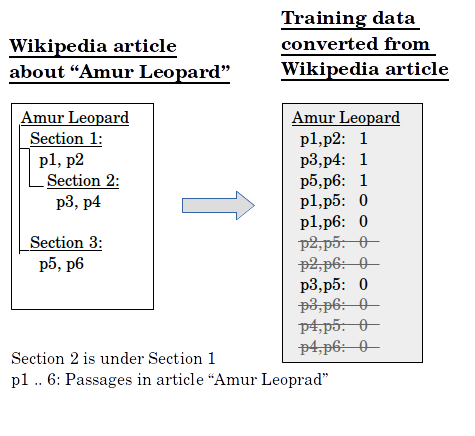
\includegraphics[width=\linewidth]{graphics/car_y1_conv.png}
  \caption{Training data generation from Article \textit{Amur Leopard} and balancing the dataset (depicted in grey strikethrough)}
  \label{fig:conv}
\end{figure}

\subsection{CATS: Context Aware Triamese Similarity network}\label{sec:cats} Similarity between a pair of texts is often subject to a context. In context of \textit{endangered species}, a pair of passages about \textit{Amur leopard} and \textit{Vaquita porpoise} should be considered similar. However this is not the case if the context changes to \textit{bycatch}. In subtopic clustering problems, context plays an important role in deciding whether passages about same broad topic should share the same subtopic cluster or not. Keeping this in mind, we propose CATS, Context Aware Triamese Similarity network, a triamese shallow network which learns a similarity function between a pair of passage embeddings given a third embedding vector containing context information. For our implementation, we use the topic title as our context information.

As depicted in Figure \ref{fig:triam}, the general CATS architecture consists of three identical fully connected triamese neural layers ($DL1$), meaning they share the same weights. Each of them accepts fixed length embedding vectors of context and pair of passages respectively ($u,v,w$). Due to their triamese nature, they project all three embedding vectors to the same embedding subspace. The projected vectors ($u',v',w'$) and their difference vectors ($(v'-w'),(v'-u'),(w'-u')$) are concatenated. The concatenated output vector is sent through another fully connected neural layer ($DL2$) which emits a similarity score.
\begin{figure}[h]
  \centering
  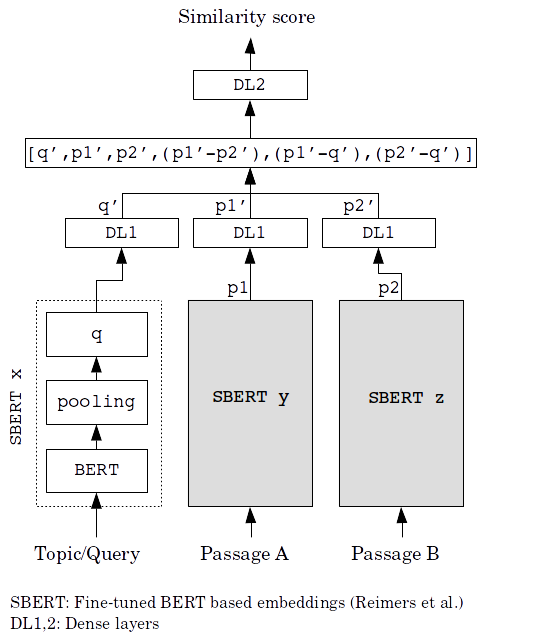
\includegraphics[width=\linewidth]{graphics/triamese.png}
  \caption{Triamese network used to estimate query dependent pairwise passage similarity score used for subtopic clustering}
  \label{fig:triam}
\end{figure}

\subsection{Finetuning transformers for sequence pair tasks} Fine-tuning is a crucial step in training Transformer models because this allows the model to be specifically suited for a particular downstream task. In the original BERT work, the BERT model is fine-tuned for a binary classification task with STSB benchmark dataset. In that work BERT model is fine-tuned for next sentence prediction task where given a sentence-pair, the model has to predict whether the second sentence should follow the first sentence. We fine-tune transformer with a modified task: given a passage-pair, predict whether they should belong to the same subtopic. This modified task setting allows us to use output of the model as the similarity score between the input passages. However, our focus for this work is to explore utilization of fixed sized passage embeddings and hence use this technique only as a strong baseline against our embedding based methods.

\section{Evaluation} 
\subsection{Experimental settings} The central theme of our work is to explore efficient way to make use of embeddings from transformer models to represent passage-length texts. Our experimental settings evaluate if such passage representations are useful in solving particularly difficult IR-centric problems involving passages. We chose sub-topic clustering of passages as our evaluation problem because traditional IR similarity metrics have been shown to be ineffective in modeling fine-grained similarity between passages about the same broad topic and hence is considered to be a difficult IR problem. However as mentioned before, we train our models to learn pairwsie distances between passages first, and then use the pairwise distances to cluster them. Following is a formal stepwise description of our clustering pipeline:
\begin{itemize}
    \item \textbf{Step 1: Binary classification} We train our model using a binary classification problem. Given a pair of passages $p_1, p_2$ from an Wikipedia article, we have to decide whether they should share the same section in that article or not. We use the TRECCAR-Train as our training data.
    \item \textbf{Step 2: Pairwise distances} Using the trained model from previous step or other unsupervised models, we calculate pairwise distances between all passage pairs which we want to cluster. If a passage embedding model is being trained (e.g. ews, ewp), then a distance function (cosine distance, CATS) is used to generate passage similarity scores between pairs of passage embedding vectors. For CATS, it is trained again for binary classification task using TRECCAR-by1train dataset.
    \item \textbf{Step 3: Subtopic clustering} Given a set of passages $P$ about a topic $T$, we have to generate $k$ clusters $c_1 .. c_k$ of passages, in such a way that each cluster $c_i$ coincides with a specific sub-topic of $T$. Using the pre-computed pairwise distances as input, we use Hierarchical Agglomerative clustering with average linkage to obtain clusters of passages from same article.
\end{itemize}

The training and evaluation phase of the clustering pipeline is depicted in Figure \ref{fig:pipe}.
\begin{figure}[h]
  \centering
  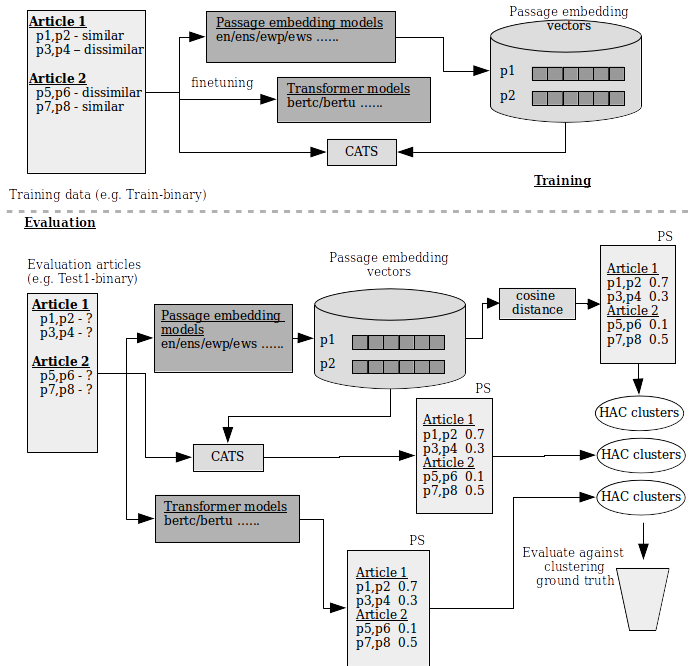
\includegraphics[width=\linewidth]{graphics/pipeline2.png}
  \caption{Training and evaluation phase of clustering pipeline}
  \label{fig:pipe}
\end{figure}

\subsection{Training and evaluation data} We use several parts of a publicly available TRECCAR dataset for training and evaluating our models: benchmarkY1-train.v2.0 (trec y1 train), benchmarkY1-test (trec y1 test), benchmarkY2test-auto-manual-qrels (trec y2 test) and train.v2.0 (trec train). The dataset consists of a large corpus of text passages extracted from Wikipedia and TQA articles. One of the target task described by the authors of the dataset is a passage retrieval task where we have to retrieve relevant passages from the corpus for complex queries. The query set is derived from concatenating section headings of an article with it's article title. For such queries, only the passages in that corresponding section of the article are considered relevant in case of automatic relevance information. This relevance information is used to obtain hierarchical structure of each articles in the dataset which are then used as input to our training data generation method depicted in Figure \ref{fig:conv}. It produces passage similarity data suitable for binary classification task and is used in step 1 (and step 2 for CATS) of our subtopic clustering pipeline.

%Each part has ground truth information contained in qrels files which inform about relevance of passages to different hierarchical sections of an Wikipedia article. For trec y1 parts, it has two different levels of hierarchical relevance: hierarchical qrels considers each section in Wikipedia articles as different topics and maps relevant passages accordingly. Toplevel qrels does not consider deeper level sections and maps all passages from deeper level sections to the section on the topmost level of the section hierarchy.

\subsubsection{Training data} Using the technique depicted in Figure \ref{fig:conv}, we convert subset of trec train and trec y1 train dataset from TRECCAR to \textbf{Train-TRECCAR} and \textbf{by1train-TRECCAR} respectively. We also generate two triplet dataset to fine-tune Dor et al. version of text embedding model. \textbf{Train-triplet-psg} contains samples of passage triplets as $(p_a, p_s, p_d)$ where $p_a$ and $p_s$ are similar and $p_d$ is dissimilar according to Train-TRECCAR. \textbf{Train-triplet-sent} is constructed similar to Train-triplet-psg except we take a random sentence from each passage in a triplet instead of the whole passage text. 

\subsubsection{Evaluation data} We evaluate our models on both binary classification task and clustering task. The former task is evaluated on \textbf{Y1 test} and \textbf{Y2 test}, converted from trec y1 test and trec y2 test, similar to \textbf{Train-TRECCAR}. For clustering task, we use section-passage relevance information from the automatic ground truth of TRECCAR dataset to construct the clustering ground truth containing true cluster of passages in articles. However, based on topical diversity inside a cluster, we construct two different clustering ground truths:

\begin{itemize}
    \item \textit{Lenient} We consider all passages under the same top-level section to be a single cluster. For example: passages relevant for \textit{Amur Leopard/Threats}, \textit{Amur Leopard/Threats/Forest degradation} and \textit{Amur Leopard/Threats/Poaching} are considered part of same \textit{"Threat"} cluster.
    \item \textit{Hierarchical} We consider passages under different hierarchical sections to be separate clusters. In previous example, we would form three distinct clusters (\textit{"Threats", "Forest degradation"} and \textit{"Poaching"}) for the \textit{"Amur Leopard"} article.
\end{itemize}

\subsection{Experimental models} We experiment with the following models:
\begin{itemize}
    \item \textbf{BERT models} BERT base cased (bert-c) and BERT base uncased (bert-u) pretrained models finetuned using Train-TRECCAR.
    \item \textbf{Passage embedding models} Four variations of Sentence-BERT models are used to generate passage embeddings: 
    \begin{itemize}
        \item \textit{en:} BERT-base model with mean-tokens pooling trained on SNLI and MultiNLI dataset.
        \item \textit{ens:} Same as en but first fine-tuned on the AllNLI datasent, then on train set of STS benchmark.
        \item \textit{ews:} Dor et al. version of text embeddings fine-tuned on triplets generated from Wikipedia sections. However to prevent training data leakage, we fine-tuned the model using Train-triplet-sent, sentence triplets generated from Train-TRECCAR, instead of the training dataset provided by the authors.
        \item \textit{ewp:} Same as ews but the model is trained on Train-triplet-psg,  passage triplets generated from Train-TRECCAR.
    \end{itemize}
    Each of the models above are used to generate passage embeddings in two ways: \textit{I. } By using the whole passage text as a single long input sequence and \textit{II. } By averaging sentence embeddings generated for each sentence of a passage. 
    \item \textbf{CATS} We train our CATS model discussed in Section \ref{sec:cats}, for each of the passage embedding methods using by1train-TRECCAR dataset. We use embedding vector of the article title as the context information for CATS.
\end{itemize}

We refer all passage embedding models by the following simple nomenclature: \texttt{EMB-GEN-DIST} where $EMB$ denotes the embedding model used ($en/ens/ews/ewp$), $GEN$ denotes whether we use the whole passage text or individual sentences as input while generating the embeddings ($psg/sent$) and finally $DIST$ denotes which type of distance function we use to obtain the similarity scores between two passage embedding vectors ($cos/CATS$).

\subsection{Subtopic clustering} For each article in \textbf{Y1 test} and \textbf{Y2 test}, we cluster all passages from the article using our clustering pipeline discussed before. The clustering results are evaluated using mean Adjusted RAND index across all the articles in each dataset. For Y1 test, we evaluate the clusters against both the \textit{lenient} and \textit{hierarchical} clustering ground truth and for Y2 test, we only evaluate on \textit{lenient} ground truth. For each case, we also evaluate two scenarios: the true number of clusters for each article is i) provided ii) not provided, so a fixed cluster number is predetermined. The supervised methods were actually trained on binary classification task, so we also report the binary classification evaluation scores in terms of AUC score (Area under the receiver operating characteristics curve). Please refer to Table \ref{tab:by1} for the evaluation results.

\begin{table*}[t]
\centering
%\ra{1.3}
\caption{Task performance measured in terms of macro averaged evaluation score and paired ttest with respect to $bertu$ with $\alpha = 0.05$}
\label{tab:by1}
\begin{tabular}{@{}lrrrrrrrrr@{}}\toprule
& \multicolumn{5}{c}{Y1 test} && \multicolumn{3}{c}{Y2 test}  \\
\cmidrule(r){2-6}
\cmidrule(r){8-10}
%\cmidrule{2-6} 
Methods & AUC & hq ARI (k=6) & hq ARI (k=true) & ln ARI (k=6) & ln ARI (k=true) && AUC & ARI (k=8) & ARI (k=true) \\\midrule
bm25 & 0.7109 & 0.0920 & 0.1771 & 0.1227 & 0.1451 && 0.6301 & 0.1571 & 0.1318 \\
LDA & & & & & && & & \\
bertc & 0.7771 & 0.1373 & 0.2300 & 0.1797 & 0.2078 && 0.6920 & 0.2275 & 0.2368 \\ 
bertu & 0.7778 & 0.1303 & 0.2140 & 0.1789 & 0.1912 && 0.6876 & 0.1824 & 0.1821 \\\midrule
ews-psg-cos & 0.7910 & 0.1451 & 0.2085 & $\blacktriangle$ 0.2302 & $\blacktriangle$ 0.2397 && $\blacktriangle$ \textbf{0.7194} & $\blacktriangle$ 0.2261 & $\blacktriangle$ 0.2422 \\ 
ewp-psg-cos & $\blacktriangle$ 0.7995 & 0.1502 & 0.2074 & $\blacktriangle$ 0.2245 & $\blacktriangle$ 0.2503 && $\blacktriangle$ 0.7089 & $\blacktriangle$ 0.2574 & $\blacktriangle$ 0.2261 \\ 
en-psg-cos & $\blacktriangledown$ 0.6686 & $\blacktriangledown$ 0.0559 & $\blacktriangledown$ 0.1018 & $\blacktriangledown$ 0.0771 & $\blacktriangledown$ 0.0910 && $\blacktriangledown$ 0.6302 & $\blacktriangledown$ 0.1041 & $\blacktriangledown$ 0.0990 \\ 
ens-psg-cos & $\blacktriangledown$ 0.6727 & $\blacktriangledown$ 0.0575 & $\blacktriangledown$ 0.1073 & $\blacktriangledown$ 0.0701 & $\blacktriangledown$ 0.0883 && $\blacktriangledown$ 0.6261 & $\blacktriangledown$ 0.0899 & $\blacktriangledown$ 0.0963 \\\midrule
ews-sent-cos & $\blacktriangledown$ 0.7379 & $\blacktriangledown$ 0.0882 & $\blacktriangledown$ 0.1564 & 0.1487 & 0.1708 && 0.6815 & 0.1515 & $\blacktriangledown$ 0.1326 \\ 
ewp-sent-cos & $\blacktriangledown$ 0.7350 & $\blacktriangledown$ 0.0951 & $\blacktriangledown$ 0.1589 & 0.1530 & 0.1663 && 0.6713 & $\blacktriangledown$ 0.1164 & $\blacktriangledown$ 0.1172 \\ 
en-sent-cos & $\blacktriangledown$ 0.6629 & $\blacktriangledown$ 0.0644 & $\blacktriangledown$ 0.1118 & $\blacktriangledown$ 0.0918 & $\blacktriangledown$ 0.0971 && $\blacktriangledown$ 0.6313 & $\blacktriangledown$ 0.1119 & $\blacktriangledown$ 0.1075 \\ 
ens-sent-cos & $\blacktriangledown$ 0.6728 & $\blacktriangledown$ 0.0598 & $\blacktriangledown$ 0.1037 & $\blacktriangledown$ 0.0856 & $\blacktriangledown$ 0.0929 && $\blacktriangledown$ 0.6280 & $\blacktriangledown$ 0.0801 & $\blacktriangledown$ 0.0797 \\\midrule
ews-psg-CATS & $\blacktriangle$ 0.7953 & $\blacktriangle$ 0.1623 & 0.2289 & $\blacktriangle$ 0.2445 & $\blacktriangle$ 0.2698 && $\blacktriangle$ 0.7173 & $\blacktriangle$ 0.2401 & $\blacktriangle$ \textbf{0.2517} \\ 
ewp-psg-CATS & $\blacktriangle$ \textbf{0.8045} & $\blacktriangle$\textbf{0.1742} & \textbf{0.2380} & $\blacktriangle$ \textbf{0.2605} & $\blacktriangle$ \textbf{0.2772} && $\blacktriangle$ 0.7097 & $\blacktriangle$ \textbf{0.2640} & $\blacktriangle$ 0.2319 \\ 
en-psg-CATS & $\blacktriangledown$ 0.7089 & 0.1106 & $\blacktriangledown$ 0.1382 & 0.1657 & 0.1608 && $\blacktriangledown$ 0.6520 & 0.1688 & 0.1623 \\ 
ens-psg-CATS & $\blacktriangledown$ 0.7094 & 0.1098 & $\blacktriangledown$ 0.1522 & 0.1561 & 0.1639 && $\blacktriangledown$ 0.6441 & 0.1533 & 0.1573 \\\midrule
ews-sent-CATS & 0.7673 & 0.1451 & 0.2041 & $\blacktriangle$ 0.2331 & $\blacktriangle$ 0.2481 && $\blacktriangle$ 0.7145 & 0.2140 & $\blacktriangle$ 0.2242 \\ 
ewp-sent-CATS & 0.7754 & 0.1539 & 0.2136 & $\blacktriangle$ 0.2314 & $\blacktriangle$ 0.2354 && 0.6995 & 0.2008 & 0.2024 \\ 
en-sent-CATS & $\blacktriangledown$ 0.7032 & $\blacktriangledown$ 0.0931 & $\blacktriangledown$ 0.1317 & $\blacktriangledown$ 0.1461 & 0.1673 && $\blacktriangledown$ 0.6572 & 0.1597 & 0.1563 \\ 
ens-sent-CATS & $\blacktriangledown$ 0.7082 & 0.1041 & $\blacktriangledown$ 0.1484 & 0.1512 & 0.1663 && $\blacktriangledown$ 0.6416 & 0.1624 & 0.1449 \\ 
\bottomrule
\end{tabular}
\caption*{Significantly higher $\blacktriangle$ or lower $\blacktriangledown$ than $bertu$ according to paired t-test \\
hq: evaluated against hierarchical clustering ground truth, ln: lenient clustering ground truth\\
k: number of clusters, k=true: original number of clusters in each article}
%\vspace{-3ex}
\end{table*}

\subsubsection{Observation} From Table \ref{tab:by1}, we make the following interesting observations:
\begin{itemize}
    \item We can see that in six out of eight cases, ewp-psg-CATS is the best performing method. All of these cases except one are statistically significant when compared to the uncased BERT method (bertu), a strong baseline, according to paired ttest.
    \item All four passage embedding methods benefit from using CATS as the distance function over cosine similarity. For example: ewp-psg-CATS improves about $15$\% over ewp-psg-CATS in terms of mean ARI score when evaluated against hierarchical ground truth of Y1 test with true number of clusters provided (column h ARI(k=true)). This improvement is not only observed for all embedding methods but across all evaluation settings as well.
    \item The CATS variant of $en, ens$ improves remarkably over their cosine similarity versions. In some cases the improvement is over $100$\%. For example: en-psg-CATS improves about $115$\% over en-psg-cos in terms of mean ARI when evaluated against lenient clustering ground truth of Y1 test with fixed number of clusters (column ln ARI(k=6)).
    \item Average sentence vector (sent) to represent passages is observed to produce worse outcome when compared to whole passage embedding (psg) for $ewp, ews$. For example: ews-sent-cos performs about $7$\% worse than ews-psg-cos in terms of AUC score for Y1 test. However, in most cases we observe slight performance increase for $en, ens$ when average sentence vector is used.
\end{itemize}

\subsubsection{Significance test} We have seen from Table \ref{tab:by1} that our proposed CATS method improves all four passage embedding methods explored here. Now to investigate whether the improvement is statistically significant, we conduct paired ttest between each CATS version of passage embedding method and it's cosine version. We choose $\alpha = 0.05$ for this study. For brevity, we consider three different cases: Y1 test with hierarchical and lenient ground truth and Y2 test, both with true number of clusters provided. We report the obtained p-value from the experiments in Table \ref{tab:sigt}. The results confirm that all improvements due to CATS are statistically significant for Y1 test dataset. Whereas for Y2 test, improvements for $en, ens$ methods are statistically significant.
\begin{table}[t]
\centering
%\ra{1.3}
\caption{Significance test of passage embedding methods with respect to it's corresponding CATS version with $\alpha = 0.05$}
\label{tab:sigt}
\begin{tabular}{@{}lrrrr@{}}\toprule
&& \multicolumn{2}{c}{Y1 test} & Y2 test  \\
\cmidrule(r){3-4}
\cmidrule(r){5-5}
Method 1 & Method 2 & hq k=t & ln k=t & k=t \\\midrule
ews-psg-cos & ews-psg-CATS & 0.0386 & 0.0138 & 0.5887 \\ 
ewp-psg-cos & ewp-psg-CATS & 0.0007 & 0.023 & 0.7462 \\ 
en-psg-cos & en-psg-CATS & 0.0002 & <0.0001 & 0.0174 \\ 
ens-psg-cos & ens-psg-CATS & <0.0001 & <0.0001 & 0.0217 \\
ews-sent-cos & ews-sent-CATS & 0.0001 & <0.0001 & 0.0004 \\
ewp-sent-cos & ewp-sent-CATS & <0.0001 & <0.0001 & 0.0016 \\
en-sent-cos & en-sent-CATS & 0.0364 & <0.0001 & 0.0684 \\
ens-sent-cos & ens-sent-CATS & 0.0001 & <0.0001 & 0.0016 \\
\bottomrule
\end{tabular}
\caption*{hq: evaluated against hierarchical clustering ground truth, ln: lenient clustering ground truth\\
k: number of clusters, k=true: original number of clusters in each article}
%\vspace{-3ex}
\end{table}

\subsubsection{Ablation study} As discussed in Section \ref{sec:cats} and Figure \ref{fig:triam}, final similarity score is learnt from the resulting vector after concatenating transformed query vector, both passage vectors and their difference vectors. To investigate the relative importance of each of these six components, we carry out an ablation study. In these study we take $ewp-psg-CATS$ and measure it's performance after removing different combinations of vectors from the concatenation step. Please refer to Table \ref{tab:abl} for the results. For brevity, we report only the three cases used for the significance test discussed previously. 

\begin{table}[t]
\centering
%\ra{1.3}
\caption{Ablation study of different components for concatenation}
\label{tab:abl}
\begin{tabular}{@{}lrrr@{}}\toprule
& \multicolumn{2}{c}{Y1 test} & Y2 test  \\
\cmidrule(r){2-3}
\cmidrule(r){4-4}
Combination & hq k=t & ln k=t & k=t \\\midrule
1. v',w' & 0.0207 & 0.0382 &  \\ 
2. v',w',(v'-w') & 0.2198 & 0.2523 & \\
3. u',v',w' & 0.0328 & 0.0415 & \\
4. u',v',w',(v'-w') & 0.2198 & 0.2690 & \\
5. u',v',w',(v'-u'),(w'-u') & 0.0359 & 0.0447 & \\
6. v',w',(v'-u'),(w'-u') & 0.0290 & 0.0434 & \\
7. v',w',(v'-w'),(v'-u'),(w'-u') & 0.2429 & 0.2795 & \\
8. (v'-w'),(v'-u'),(w'-u') & 0.2193 & 0.2639 & \\
9. (v'-u'),(w'-u') & 0.0281 & 0.0469 & \\
\textbf{10. u',v',w',(v'-w'),(v'-u'),(w'-u')} & 0.2380 & 0.2772 & 0.2319 \\
\bottomrule
\end{tabular}
\caption*{Bold text refers to the combination used for our experiments \\
u',v',w': Refer to Figure \ref{fig:triam}}
%\vspace{-3ex}
\end{table}

From the result we can make the following observations:
\begin{itemize}
    \item Combination 1 and 2 do not involve context vector (u') and both of them performs worse than many other combinations involving context vector. Hence we can conclude that including context vector positively impacts model's ability to estimate topical similarity between passage embedding vectors.
    \item Another interesting observation we make from Table \ref{tab:abl} is the fact that difference vectors are more helpful than original embedding vector. For example, inclusion of the difference vector between two passage embedding vectors (v'-w') in Combination 4 along with all three embedding vectors (u',v',w') resulted in large performance gain over Combination 3. In fact Combination 8 which uses only the difference vectors, yields comparable results with best performing methods.
    \item We observe that Combination 7 obtains slightly better results than Combination 10 (all six components) which is used for our clustering study. This suggests that the success of CATS comes from the difference vectors between passage and context and not from the context vector itself. 
\end{itemize}

As discussed before, we use the title of articles as our context information. Thus it is only natural to find topical similarity between the article title and any passage from the article. So while estimating subtopic similarity between these passages, the deciding factors should be other topics than the title topic (context) which is represented by the difference vector between passage and context. We find evidence for this in our ablation study as it showed difference vectors to be more beneficial. 

\subsection{Qualitative study} We conduct a qualitative analysis on the clustering evaluation. The aim of this analysis is to explain why some of the methods we present here are better than the rest and to provide example cases from the dataset bolstering the explanation.

Consider the following pair of passages from Y1 test dataset:

\noindent\fbox{%
    \parbox{0.48\textwidth}{%
        \textbf{Passage 1: } Gardens in Renaissance were adorned with sculptures, topiary and fountains. In the 17th century, knot gardens became popular along with the hedge mazes. By this time, Europeans started planting new flowers such as tulips, marigolds and sunflowers. \\
        \textbf{Passage 2: } Islamic gardens were built after the model of Persian gardens and they were usually enclosed by walls and divided in 4 by watercourses. Commonly, the center of the garden would have a pool or pavilion. Specific to the Islamic gardens are the mosaics and glazed tiles used to decorate the rills and fountains that were built in these gardens.
    }%
}

From only the text of the passages, it is quite difficult to decide whether they are similar enough to share same subtopic cluster. In context of human culture they are topically distinct but in context of history of gardening, they are similar. Due to this ambiguity, $en-psg-cos$, which does not have access to the context information, assigned low similarity score to this passage pair. But the passage pair is taken from the Y1 test article titled \textit{"Gardening"} and share the \textit{"History (of gardening)"} subtopic. Access to this piece of information (article title) helps the CATS variant $en-psg-CATS$ to resolve the ambiguity and as a result it is able to correctly assign high similarity scores between them.

The previous example is a case of false negative which is rectified by CATS approach. However, we find this to be rare instance across both the datasets and embedding methods. The dominant reason for CATS approach to achieve better results is it's ability to identify false positive cases. Let us consider another pair of passages again from Y1 test dataset:

\noindent\fbox{%
    \parbox{0.48\textwidth}{%
        \textbf{Passage 1: } Big-game fishing started as a sport after the invention of the motorized boat.  In 1898, Dr. Charles Frederick Holder, a marine biologist and early conservationist, pioneered this sport and went on to publish many articles and books on the subject noted for their combination of accurate scientific detail with exciting narratives. \\
        \textbf{Passage 2: } In addition to capturing fish for food, recreational anglers might also keep a log of fish caught, either in a physical form or with technology such as the FISHBUOY or Fishbrain mobile logging application, and submit trophy-sized fish to independent record keeping bodies. In the Republic of Ireland, the Irish Specimen Fish Committee ...... It also uses a set of 'fair play' regulations to ensure fish are caught in accordance with accepted angling norms.
    }%
}

It is evident that these two passages share topics such as \textit{"fishing"}, \textit{"sport"} and consequently influence non-CATS method such as $ewp-psg-cos$ to incorrectly assign high similarity score. However, when we are aware that both these passages are taken from an article titled \textit{"Recreational fishing"}, then other less overt topics become more important in deciding their subtopic similarity. As there are little topical overlap other than the central context, $ewp-psg-cos$ assigns low similarity score for the pair. Indeed these two passages are taken from different subtopics, \textit{"History"} and \textit{"Fish logs"} respectively. 

\subsection{Effect of post-processing and dimensionality reduction} Mu et al. had shown us that much of the variance of popular word embedding vectors are explained by only a small subset of vector dimensions. In their study, they develop a simple post-processing technique which made the embeddings stronger by eliminating those dominating embedding dimensions, as opposed to eliminating the weakest dimensions in case of typical dimensionality reduction techniques. According to their findings, their technique can be used to initialize embedding vectors for supervised downstream tasks. However, when used with our best performing CATS variant $q-ewp$, it does not yield any significant improvement.

All passage embeddings used for our evaluation are of length 768. Reducing the dimensionality of embeddings without significantly hurting the performance, benefit memory-constrained downstream applications. Raunak et al. propose a dimensionality reduction technique that combines PCA with Mu et al. post-processing algorithm, suitable for word embeddings. We explore the applicability of their technique to passage embeddings in comparison to simple PCA. Our findings, presented in Figure \ref{fig:dimred}, lead to interesting insights. As expected, for $ewp$ and $ews$, reducing dimensionality using normal PCA degrades performance in terms of AUC score for binary classification task. However, the performance degradation is much more when we apply the technique by Raunak et al. On the other hand, for $en$ and $ens$, reduced embedding vectors produce improved results compared to the original vector. More interestingly, the improvement sustains even if the embedding size is reduced to only 100. Our conclusions from this observation are as follows:
\begin{itemize}
    \item The key difference between $en, ens$ and $ewp, ews$ is the incorporation of Wikipedia section information for the later two. The dimensionality reduction technique by Raunak et al. eliminates dominating dimensions similar to Mu et al. and eliminates weakest dimensions using PCA. As our evaluation results show, applying Raunak et al. method hurts the performance much more than a simple PCA dimensionality reduction. This suggests that important Wikipedia hierarchy information is concentrated in dominant dimensions of these passage embeddings and when those dimensions are eliminated, the performance degradation is much severe than simple PCA.
    \item For $en, ens$, dimensionality reduction results in improved performance and the improvement is slightly higher for Raunak et al. This finding aligns with the work of Mu et al. and Raunak et al. with word embeddings. Unlike $ewp, ews$, these embeddings do not have essential information concentrated in specific sets of dimensions and hence do not lose important insights upon removal of dominant or weak dimensions. In fact they benefit from denoising nature of these post-processing techniques.
\end{itemize}

\begin{figure}[h]
  \centering
  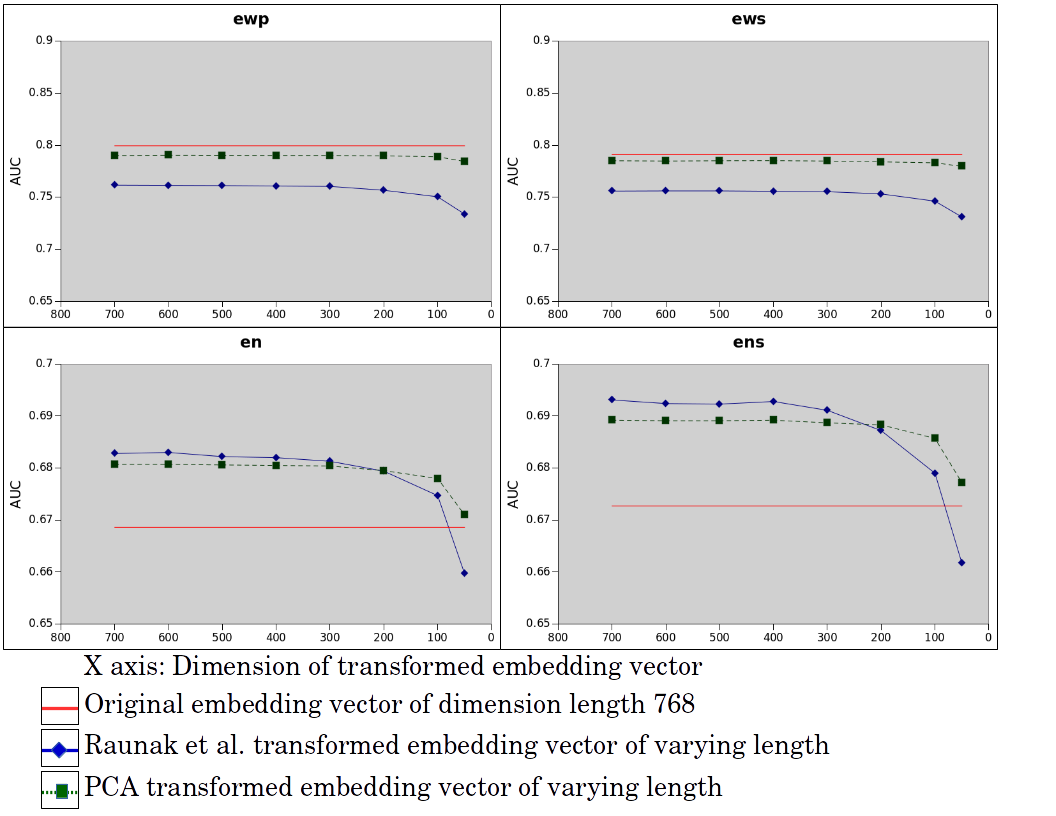
\includegraphics[width=\linewidth]{graphics/emb_vec_dim_red_exp.png}
  \caption{Effect of dimensionality reduction of passage embedding vectors compared to the original vector}
  \label{fig:dimred}
\end{figure}

\section{Conclusion} Transformer based embedding models have been applied successfully solve sentence or phrase similarity tasks. On the other hand, to solve difficult IR-centric problems such as subtopic clustering, we require contextual understanding of long-form texts that Transformer models such as BERT can provide. But several engineering limitations prevented usage of these models for longer sequence of texts such as passage or documents. We develop simple yet powerful techniques to adapt Transformer based embedding models to generate passage embeddings, suitable for capturing subtopic similarity. We also propose CATS, a Triamese neural architecture that models contextual similarity function between passage embedding vectors. Our exhaustive empirical findings show that our Transformer based passage embeddings in tandem with CATS, outperform strong BERT baseline models and therefore can be used as a simple and better solution to the subtopic clustering problems.

\bibliographystyle{plain}
\bibliography{myref}
\end{document}
\endinput
%%
%% End of file `sample-authordraft.tex'.
